\section{Geometrical classifiers}

\subsection{Ellipsoids array classifier}

The construction of a classifier using array of identifiers is pretty simple and straightforward. The array is filled with ellipsoids, one for each class in the training dataset. Every unknown pattern, sent for classification, moves through those ellipsoids and gets the information whether it lies inside the ellipsoid or not. In case of being part of identifier's interior the value given by the equation (\ref{eq:ellipsoid_affiliation}) is taken into consideration, which tells about the position inside the ellipsoid (where value 0 means that the point is in the ellipsoid's centre and 1 means that it lies on the surface). Finally, after all ellipsoids are checked, the one with the smallest equation (\ref{eq:ellipsoid_affiliation}) value (and for which the point lies inside it), designates the class to which this unknown pattern should be classified to. If no ellipsoid accepts the point, it is rejected and treated as a foreign element. 

One way of increasing rejection ratio would be to decrease ellipsoid size. The smaller the volume the less points lie inside, which in turn boosts rejection rates but worsens classification. Changing ellipsoid size can be helpful in a situation in which two classes overlap and rejection of the elements is more desired result than misclassification.

\begin{figure}[htp]
	\centering
	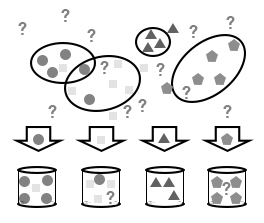
\includegraphics[width=0.8\textwidth]{Figures/ellipsoid_classification.jpg}
	\caption{ Array of ellipsoids that works as a classifier with rejection capabilities. Elements outside of existing ellipsoids are treated as a foreign patterns. Those within ellipsoids are classified as native patterns. }
	\label{fig:ellipsoids_array}\vspace{-3pt}
\end{figure}

\subsection{Optimizing ellipsoid size} \ \label{size_optimizing}

One thing worth noting when using ellipsoids is that their size can be easily enlarged when having few points that are located far away from their class centre. This situation can lead to decrease in rejection option rates as well as bigger misclassification between native elements' classes. Of course decreasing ellipsoid size can result in the opposite situation. The key to deal with this difficulty is to find balance between decreasing ellipsoid size and still getting high rejection and classification rates. Two approaches are proposed in this paper.

\subsubsection{Tolerance parameter manipulation}

The tolerance parameter, also named as $\varepsilon$ in Equation (\ref{eq:ellipsoid_affiliation}), can be used during point affiliation check-up to manipulate the result of the equation. By decreasing its value the ellipsoid ``shrinks`` evenly in all directions, and by increasing it more points are accepted as if they were lying inside the ellipsoid. Overall 100 tests there were performed with $\varepsilon$ consecutive values being~$(1, 0.98, 0.96, \dots, -0.98)$. The results can be seen in Figure \ref{fig:shrinking_ellipsoids_tolerance_manipulation}. The identification measurement corresponds to the number of native elements from outside of the examined class that were incorrectly classified (identified) by the ellipsoid. The lower the value, the better. The relationship between number of correctly classified native elements and properly rejected foreigners can be seen in Figure \ref{fig:shrinking_ellipsoids_tolerance_manipulation2}.

\begin{figure}[htp]
	\centering
	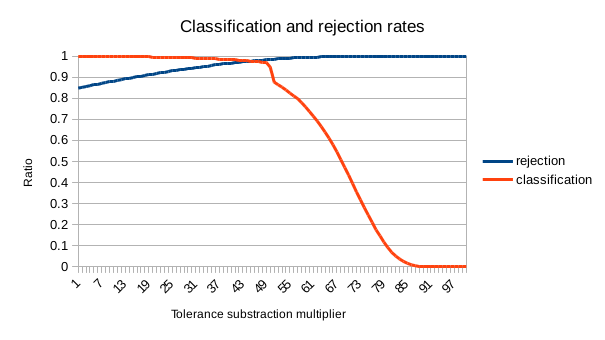
\includegraphics[width=1.\textwidth]{Figures/shrinking_ellipsoid_tolerance_manipulation.png}
	\caption{ Classification and rejection rates for different $\varepsilon$ values. Classification value corresponds to the number of native elements from the tested class that were correctly classified. Identification informs about number of native elements from other classes that were incorrectly classified (identified) by the ellipsoid. Rejection value informs about correctly rejected foreign patterns. Bigger classification and rejection values and smaller identification are better. }
	\label{fig:shrinking_ellipsoids_tolerance_manipulation}\vspace{-3pt}
\end{figure}

\begin{figure}[htp]
\centering
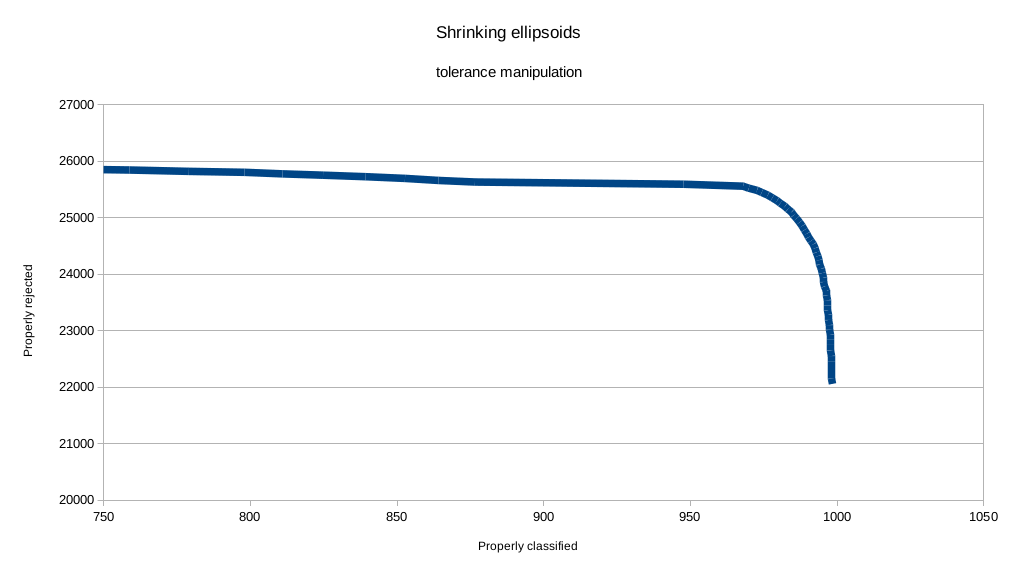
\includegraphics[width=1.\textwidth]{Figures/shrinking_ellipsoid_tolerance_manipulation2.png}
\caption{ Relationship of classified and rejected points in the shrinking ellipsoids using tolerance modification approach. }
\label{fig:shrinking_ellipsoids_tolerance_manipulation2}\vspace{-3pt}
\end{figure}

\subsubsection{Native elements removal}

The problem with manipulating the tolerance parameter is that the shape of the ellipsoid stays the same for the whole time. This is not a desired solution in a situation in which some of the patterns are located far from the rest of native elements in the same class, which results in bigger ellipsoid but mostly empty inside. In such case it should be better to ignore those points and prefer smaller volume ellipsoid with worse classification capabilities. This approach has been tested by checking classification and rejection rates for ellipsoids built on increasingly smaller datasets. Each step of the shrinking ellipsoid algorithm consists of creating ellipsoid for certain number of patterns. Those elements are sorted base on the inclusion testing function value (Equation \ref{eq:ellipsoid_affiliation}), and 5 most distant ones are removed from the set. The classification and rejection rates are obtained based on the new ellipsoid created on this smaller set and the whole procedure is repeated. The results of this algorithm, which can be seen in Figure \ref{fig:shrinking_ellipsoids_elements_rejection}, were obtained for 100 steps which resulted (in the 100th step) in 495 elements removed from the original data set. The correlation between number of properly classified native elements and rejected foreign patterns can be seen on the Figure \ref{fig:shrinking_ellipsoids_elements_rejection2}.

\begin{figure}[htp]
	\centering
	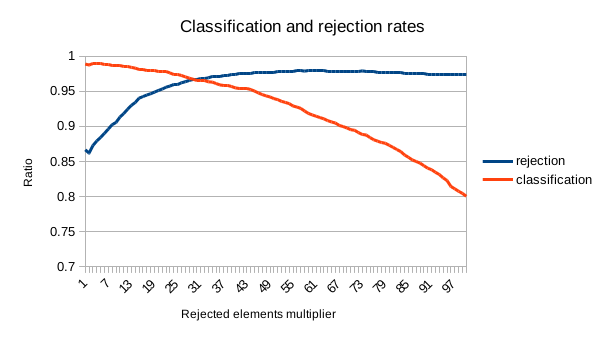
\includegraphics[width=1.\textwidth]{Figures/shrinking_ellipsoid_elements_rejection.png}
	\caption{ Classification and rejection rates for each native element removal step. In each step 5 elements were deleted from the set resulting in overall 500 elements removed in the final 100th step. Identification informs about number of native elements from other classes that were incorrectly classified (identified) by the ellipsoid. Rejection value informs about correctly rejected foreign patterns. Bigger classification and rejection values and smaller identification are better. }
	\label{fig:shrinking_ellipsoids_elements_rejection}\vspace{-3pt}
\end{figure}

\begin{figure}[htp]
	\centering
	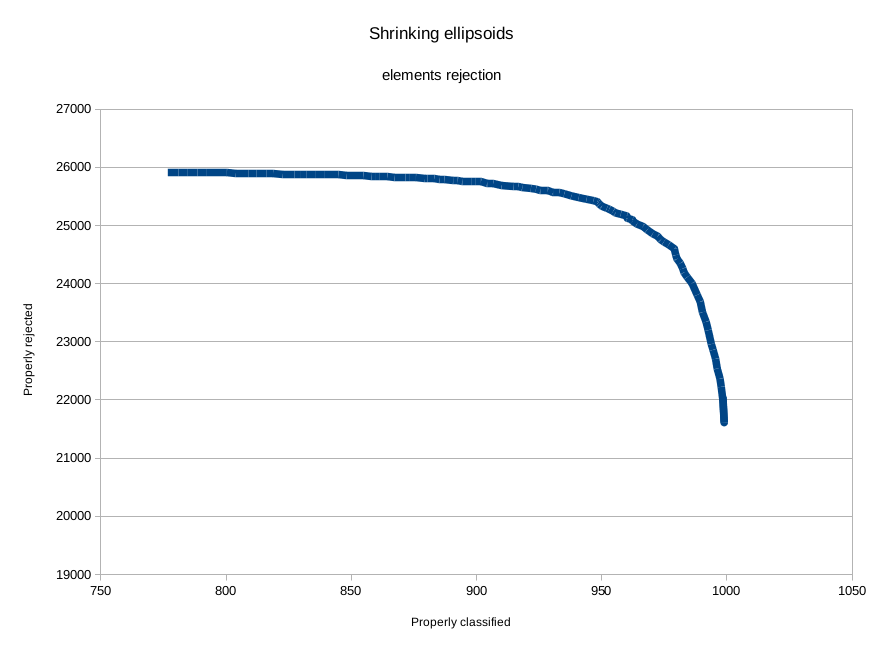
\includegraphics[width=1.\textwidth]{Figures/shrinking_ellipsoid_elements_rejection2.png}
	\caption{ Relationship of classified and rejected points in the shrinking ellipsoids using element removal approach. }
	\label{fig:shrinking_ellipsoids_elements_rejection2}\vspace{-3pt}
\end{figure}

\subsection{Summary}

The tests performed on the classifier using array of identifiers prove that it can successfully combine classification and rejection tasks. While being unable to do the multi-class classification on their own, combined ellipsoids can be very accurate at classification and rejecting foreigners. Minimum volume enclosing ellipsoids combine advantages of commonly used classifiers described in Chapter \ref{common_classifiers} such as easy point inclusion detection, and iterative construction algorithm that uses tolerance parameter for its stop condition. The main disadvantage of ellipsoid, and minimum volume enclosing figures in general, is the fact that it does not transform the feature space of presented data. In order to get good results the data should be separable, and no generalisation of information is done at all. This is completely different from the attitude introduced in random forest or svm.
